\documentclass[../notes.tex]{subfiles}
\graphicspath{{\subfix{../images/}}, {\subfix{../}}}

\begin{document}

\chapter{Superconductivity}\label{ch:superconductivity}

Superconductivity is an example of an emergent phenomenon: the Schrödinger equation describing all interactions between electrons gives no indication that there exists parameters for which the electrons condense into phase coherent pairs.
In this chapter we review theoretical concepts needed for understanding superconductivity and introduce the tools used to study superconductivity in the later chapters.
There are many textbooks covering these topics which can be referenced for a more detailed treatment, such as refs. \cite{colemanIntroductionManyBodyPhysics2015, tinkhamIntroductionSuperconductivity1996, bruusManyBodyQuantumTheory2004, larkinTheoryFluctuationsSuperconductors2005, bennemannSuperconductivity2008}.

Macroscopially, the superconducting state can be described by a spontaneous breaking of a \(U(1)\) phase rotation symmetry that is associated with an order parameter.
Theory of spontaneous symmetry breaking and associated phase transitions is Ginzburg-Landau theory discussed in \cref{sec:Ginzburg-Landau theory of superconductivity}.
\todo{Talk about finite q specifically!}

Ginzburg Landau theory is not a macroscopic theory, but it can be connected to microscopic theories: if a theory finds an expression for the order parameter describing the symmetry breakdown, it can be connected to quantities expressed by Ginzburg-Landau theory, such as the superconducting current.
One such theory to describe superconductivity from a microscopic perspective is \acrfull{bcs} theory in \cref{sec:bcs-theory}.

A method to treat local interactions non-perturbatively is \acrfull{dmft}. \Cref{sec:Dynamical Mean-Field Theory} briefly introduces the Greens function method to treat many-body problems and outlines the \acrshort{dmft} self-consistency cycle.

\section{Ginzburg-Landau Theory of Superconductivity}\label{sec:Ginzburg-Landau theory of superconductivity}

This review partially follows the introduction given in refs.~\cite{colemanIntroductionManyBodyPhysics2015, beekmanIntroductionSpontaneousSymmetry2019}.

\paragraph{\acrlong{ssb}}

Symmetries are a powerful concept in physics.
Noethers theorem \cite{noetherInvarianteVariationsprobleme1918} connects the symmetries of physical theories to associated conservation laws.
An interesting facet of symmetries in physical theories is the fact, that a ground state of a system must not necessarily obey the same symmetries of its Hamiltonian, i.e. for a symmetry operation that is described by a unitary operator \(U\), the Hamiltonian commutes with \(U\) (which results in expectation values of the Hamiltonian being invariant under the symmetry operation) but the states \(\ket{\phi}\) and \(U \ket{\phi}\) are different.
This phenomenon is called \acrfull{ssb} and the state \(\ket{\phi}\) is said to be symmetry-broken.

One consequence of this fact is that for a given symmetry-broken state \(\ket{\phi}\), there exists multiple states that can be reached by repeatedly applying \(U\) to \(\ket{\phi}\) and all have the same energy.
To differentiate the symmetry-broken states an operator can be defined that has all these equivalent states as eigenvectors with different eigenvalues and zero expectation value for symmetric states.
This is the microscopic notion of an order parameter.

\paragraph{Order parameter}

The original notion of an order parameter was motivated from macroscopic observables that can then be related to the microscopic order parameter operator introduced above.
Macroscopically we characterize the symmetry breaking by an order parameter \(\Psi\) which generally can be a complex-valued vector that becomes non-zero below the transition temperature \(T_C\):
\begin{equation}
	\vert \Psi \vert =
	\begin{cases}
		0 & T > T_C \\
		\vert \Psi_0 \vert > 0 & T < T_C
	\end{cases} \;.
\end{equation}
In the example of a ferromagnet, a finite measurable magnetization of a material is associated with a finite expectation value for the \(z\)-component of the spin operator, \(m_z = \braket{\ope{S_z}}\).
This \cite{landauTheoryPhaseTransitions1937}

\todo{Work over paragraph}

Similarly to a magnetically ordered state, the SC state is characterized by 

\cite{ginzburgTheorySuperconductivity1950}

\todo{Order parameters from observables -> in contrast to microscopic OP}

Ginzburg-Landau theory is concerned with the the properties of the 

It does not need microscopic expression for order parameter, it provides corse-grained description of the properties of matter.
The order parameter description is good at length scales above \(\xi_0\), the coherence length (e.g.\ size of Cooper pairs for SC).
On length scales above \(\xi_0\), the order parameter behaves as a smoothly varying function.

\paragraph{Landau theory} \todo{Work over paragraph}

Basic idea of Landau theory: write free energy as function \(F[\psi]\) of the order parameter.
Region of small \(\psi\), expand free energy of many-body system as simple polynomial:
\begin{equation}
	f_{L} = \frac{1}{V} F[\psi] = \frac{r}{2} \psi^2 + \frac{u}{4} \psi^4
\end{equation}
Provided \(r\) and \(u\) are greater that \(0\): minimum of \(f_L [\psi])\) lies at \(\psi = 0\).
Landau theory assumes: at phase transition temperature \(r\) changes sign, so:
\begin{equation}
	r = a(T - T_C)
\end{equation}
Minimum of free energy occurs for:
\begin{equation}
	\psi = \begin{cases}
		0 \\
		\pm \sqrt{\frac{a (T_C - T)}{u} }
	\end{cases}
\end{equation}

\todo{Make graphic for Landau free energy}

\todo{Make graphic for Landau OP and BCS OP}

\todo{Make my own graphic for mexican hat potential}

\begin{figure}[t]
	\centering
	\begin{subfigure}[b]{0.5\textwidth}
			\centering
			%% Creator: Matplotlib, PGF backend
%%
%% To include the figure in your LaTeX document, write
%%   \input{<filename>.pgf}
%%
%% Make sure the required packages are loaded in your preamble
%%   \usepackage{pgf}
%%
%% Also ensure that all the required font packages are loaded; for instance,
%% the lmodern package is sometimes necessary when using math font.
%%   \usepackage{lmodern}
%%
%% Figures using additional raster images can only be included by \input if
%% they are in the same directory as the main LaTeX file. For loading figures
%% from other directories you can use the `import` package
%%   \usepackage{import}
%%
%% and then include the figures with
%%   \import{<path to file>}{<filename>.pgf}
%%
%% Matplotlib used the following preamble
%%   \def\mathdefault#1{#1}
%%   \everymath=\expandafter{\the\everymath\displaystyle}
%%   \IfFileExists{scrextend.sty}{
%%     \usepackage[fontsize=10.000000pt]{scrextend}
%%   }{
%%     \renewcommand{\normalsize}{\fontsize{10.000000}{12.000000}\selectfont}
%%     \normalsize
%%   }
%%   \usepackage{fontspec}\usepackage{unicode-math}\setmathfont{texgyrepagella-math.otf}\setmainfont{texgyrepagella-math}
%%   \makeatletter\@ifpackageloaded{underscore}{}{\usepackage[strings]{underscore}}\makeatother
%%
\begingroup%
\makeatletter%
\begin{pgfpicture}%
\pgfpathrectangle{\pgfpointorigin}{\pgfqpoint{2.252757in}{2.135967in}}%
\pgfusepath{use as bounding box, clip}%
\begin{pgfscope}%
\pgfsetbuttcap%
\pgfsetmiterjoin%
\definecolor{currentfill}{rgb}{1.000000,1.000000,1.000000}%
\pgfsetfillcolor{currentfill}%
\pgfsetlinewidth{0.000000pt}%
\definecolor{currentstroke}{rgb}{1.000000,1.000000,1.000000}%
\pgfsetstrokecolor{currentstroke}%
\pgfsetdash{}{0pt}%
\pgfpathmoveto{\pgfqpoint{0.000000in}{0.000000in}}%
\pgfpathlineto{\pgfqpoint{2.252757in}{0.000000in}}%
\pgfpathlineto{\pgfqpoint{2.252757in}{2.135967in}}%
\pgfpathlineto{\pgfqpoint{0.000000in}{2.135967in}}%
\pgfpathlineto{\pgfqpoint{0.000000in}{0.000000in}}%
\pgfpathclose%
\pgfusepath{fill}%
\end{pgfscope}%
\begin{pgfscope}%
\pgfsetbuttcap%
\pgfsetmiterjoin%
\definecolor{currentfill}{rgb}{1.000000,1.000000,1.000000}%
\pgfsetfillcolor{currentfill}%
\pgfsetlinewidth{0.000000pt}%
\definecolor{currentstroke}{rgb}{0.000000,0.000000,0.000000}%
\pgfsetstrokecolor{currentstroke}%
\pgfsetstrokeopacity{0.000000}%
\pgfsetdash{}{0pt}%
\pgfpathmoveto{\pgfqpoint{0.050000in}{0.050000in}}%
\pgfpathlineto{\pgfqpoint{2.057250in}{0.050000in}}%
\pgfpathlineto{\pgfqpoint{2.057250in}{2.044300in}}%
\pgfpathlineto{\pgfqpoint{0.050000in}{2.044300in}}%
\pgfpathlineto{\pgfqpoint{0.050000in}{0.050000in}}%
\pgfpathclose%
\pgfusepath{fill}%
\end{pgfscope}%
\begin{pgfscope}%
\definecolor{textcolor}{rgb}{0.000000,0.000000,0.000000}%
\pgfsetstrokecolor{textcolor}%
\pgfsetfillcolor{textcolor}%
\pgftext[x=2.197758in,y=0.887606in,,top]{\color{textcolor}{\rmfamily\fontsize{10.000000}{12.000000}\selectfont\catcode`\^=\active\def^{\ifmmode\sp\else\^{}\fi}\catcode`\%=\active\def%{\%}$\Psi$}}%
\end{pgfscope}%
\begin{pgfscope}%
\pgfpathrectangle{\pgfqpoint{0.050000in}{0.050000in}}{\pgfqpoint{2.007250in}{1.994300in}}%
\pgfusepath{clip}%
\pgfsetrectcap%
\pgfsetroundjoin%
\pgfsetlinewidth{1.003750pt}%
\definecolor{currentstroke}{rgb}{0.800000,0.400000,0.466667}%
\pgfsetstrokecolor{currentstroke}%
\pgfsetdash{}{0pt}%
\pgfpathmoveto{\pgfqpoint{0.192273in}{2.054300in}}%
\pgfpathlineto{\pgfqpoint{0.210719in}{1.899358in}}%
\pgfpathlineto{\pgfqpoint{0.232660in}{1.730734in}}%
\pgfpathlineto{\pgfqpoint{0.254601in}{1.578217in}}%
\pgfpathlineto{\pgfqpoint{0.276542in}{1.440873in}}%
\pgfpathlineto{\pgfqpoint{0.298484in}{1.317791in}}%
\pgfpathlineto{\pgfqpoint{0.320425in}{1.208089in}}%
\pgfpathlineto{\pgfqpoint{0.342366in}{1.110906in}}%
\pgfpathlineto{\pgfqpoint{0.360650in}{1.038882in}}%
\pgfpathlineto{\pgfqpoint{0.378934in}{0.974504in}}%
\pgfpathlineto{\pgfqpoint{0.397219in}{0.917315in}}%
\pgfpathlineto{\pgfqpoint{0.415503in}{0.866871in}}%
\pgfpathlineto{\pgfqpoint{0.433787in}{0.822739in}}%
\pgfpathlineto{\pgfqpoint{0.452072in}{0.784499in}}%
\pgfpathlineto{\pgfqpoint{0.470356in}{0.751744in}}%
\pgfpathlineto{\pgfqpoint{0.488640in}{0.724078in}}%
\pgfpathlineto{\pgfqpoint{0.506925in}{0.701116in}}%
\pgfpathlineto{\pgfqpoint{0.521552in}{0.685885in}}%
\pgfpathlineto{\pgfqpoint{0.536179in}{0.673243in}}%
\pgfpathlineto{\pgfqpoint{0.550807in}{0.663010in}}%
\pgfpathlineto{\pgfqpoint{0.565434in}{0.655012in}}%
\pgfpathlineto{\pgfqpoint{0.580062in}{0.649080in}}%
\pgfpathlineto{\pgfqpoint{0.598346in}{0.644320in}}%
\pgfpathlineto{\pgfqpoint{0.616630in}{0.642220in}}%
\pgfpathlineto{\pgfqpoint{0.634915in}{0.642484in}}%
\pgfpathlineto{\pgfqpoint{0.653199in}{0.644824in}}%
\pgfpathlineto{\pgfqpoint{0.675140in}{0.649989in}}%
\pgfpathlineto{\pgfqpoint{0.700738in}{0.658700in}}%
\pgfpathlineto{\pgfqpoint{0.729993in}{0.671380in}}%
\pgfpathlineto{\pgfqpoint{0.766562in}{0.689970in}}%
\pgfpathlineto{\pgfqpoint{0.898208in}{0.759831in}}%
\pgfpathlineto{\pgfqpoint{0.931120in}{0.773608in}}%
\pgfpathlineto{\pgfqpoint{0.960375in}{0.783559in}}%
\pgfpathlineto{\pgfqpoint{0.989630in}{0.791040in}}%
\pgfpathlineto{\pgfqpoint{1.015228in}{0.795389in}}%
\pgfpathlineto{\pgfqpoint{1.040826in}{0.797587in}}%
\pgfpathlineto{\pgfqpoint{1.066424in}{0.797587in}}%
\pgfpathlineto{\pgfqpoint{1.092022in}{0.795389in}}%
\pgfpathlineto{\pgfqpoint{1.117620in}{0.791040in}}%
\pgfpathlineto{\pgfqpoint{1.143218in}{0.784635in}}%
\pgfpathlineto{\pgfqpoint{1.172473in}{0.774978in}}%
\pgfpathlineto{\pgfqpoint{1.205385in}{0.761482in}}%
\pgfpathlineto{\pgfqpoint{1.241953in}{0.743846in}}%
\pgfpathlineto{\pgfqpoint{1.289492in}{0.718241in}}%
\pgfpathlineto{\pgfqpoint{1.366286in}{0.676702in}}%
\pgfpathlineto{\pgfqpoint{1.399198in}{0.661631in}}%
\pgfpathlineto{\pgfqpoint{1.424796in}{0.652210in}}%
\pgfpathlineto{\pgfqpoint{1.446737in}{0.646280in}}%
\pgfpathlineto{\pgfqpoint{1.468679in}{0.642794in}}%
\pgfpathlineto{\pgfqpoint{1.486963in}{0.642093in}}%
\pgfpathlineto{\pgfqpoint{1.505247in}{0.643697in}}%
\pgfpathlineto{\pgfqpoint{1.523531in}{0.647901in}}%
\pgfpathlineto{\pgfqpoint{1.538159in}{0.653342in}}%
\pgfpathlineto{\pgfqpoint{1.552786in}{0.660808in}}%
\pgfpathlineto{\pgfqpoint{1.567414in}{0.670466in}}%
\pgfpathlineto{\pgfqpoint{1.582041in}{0.682489in}}%
\pgfpathlineto{\pgfqpoint{1.596669in}{0.697056in}}%
\pgfpathlineto{\pgfqpoint{1.611296in}{0.714350in}}%
\pgfpathlineto{\pgfqpoint{1.625923in}{0.734558in}}%
\pgfpathlineto{\pgfqpoint{1.644208in}{0.764214in}}%
\pgfpathlineto{\pgfqpoint{1.662492in}{0.799115in}}%
\pgfpathlineto{\pgfqpoint{1.680776in}{0.839661in}}%
\pgfpathlineto{\pgfqpoint{1.699061in}{0.886267in}}%
\pgfpathlineto{\pgfqpoint{1.717345in}{0.939356in}}%
\pgfpathlineto{\pgfqpoint{1.735629in}{0.999367in}}%
\pgfpathlineto{\pgfqpoint{1.753914in}{1.066748in}}%
\pgfpathlineto{\pgfqpoint{1.772198in}{1.141961in}}%
\pgfpathlineto{\pgfqpoint{1.790482in}{1.225480in}}%
\pgfpathlineto{\pgfqpoint{1.812423in}{1.337352in}}%
\pgfpathlineto{\pgfqpoint{1.834364in}{1.462749in}}%
\pgfpathlineto{\pgfqpoint{1.856306in}{1.602558in}}%
\pgfpathlineto{\pgfqpoint{1.878247in}{1.757694in}}%
\pgfpathlineto{\pgfqpoint{1.900188in}{1.929095in}}%
\pgfpathlineto{\pgfqpoint{1.914977in}{2.054300in}}%
\pgfpathlineto{\pgfqpoint{1.914977in}{2.054300in}}%
\pgfusepath{stroke}%
\end{pgfscope}%
\begin{pgfscope}%
\pgfpathrectangle{\pgfqpoint{0.050000in}{0.050000in}}{\pgfqpoint{2.007250in}{1.994300in}}%
\pgfusepath{clip}%
\pgfsetrectcap%
\pgfsetroundjoin%
\pgfsetlinewidth{1.003750pt}%
\definecolor{currentstroke}{rgb}{0.200000,0.133333,0.533333}%
\pgfsetstrokecolor{currentstroke}%
\pgfsetdash{}{0pt}%
\pgfpathmoveto{\pgfqpoint{0.141239in}{1.148426in}}%
\pgfpathlineto{\pgfqpoint{0.163180in}{0.988971in}}%
\pgfpathlineto{\pgfqpoint{0.185121in}{0.847129in}}%
\pgfpathlineto{\pgfqpoint{0.207062in}{0.721885in}}%
\pgfpathlineto{\pgfqpoint{0.225346in}{0.629479in}}%
\pgfpathlineto{\pgfqpoint{0.243631in}{0.547353in}}%
\pgfpathlineto{\pgfqpoint{0.261915in}{0.474958in}}%
\pgfpathlineto{\pgfqpoint{0.280199in}{0.411761in}}%
\pgfpathlineto{\pgfqpoint{0.298484in}{0.357239in}}%
\pgfpathlineto{\pgfqpoint{0.316768in}{0.310880in}}%
\pgfpathlineto{\pgfqpoint{0.331395in}{0.279336in}}%
\pgfpathlineto{\pgfqpoint{0.346023in}{0.252449in}}%
\pgfpathlineto{\pgfqpoint{0.360650in}{0.229973in}}%
\pgfpathlineto{\pgfqpoint{0.375278in}{0.211670in}}%
\pgfpathlineto{\pgfqpoint{0.389905in}{0.197305in}}%
\pgfpathlineto{\pgfqpoint{0.404532in}{0.186648in}}%
\pgfpathlineto{\pgfqpoint{0.419160in}{0.179474in}}%
\pgfpathlineto{\pgfqpoint{0.430131in}{0.176249in}}%
\pgfpathlineto{\pgfqpoint{0.441101in}{0.174769in}}%
\pgfpathlineto{\pgfqpoint{0.455729in}{0.175356in}}%
\pgfpathlineto{\pgfqpoint{0.470356in}{0.178681in}}%
\pgfpathlineto{\pgfqpoint{0.484983in}{0.184542in}}%
\pgfpathlineto{\pgfqpoint{0.499611in}{0.192741in}}%
\pgfpathlineto{\pgfqpoint{0.517895in}{0.205988in}}%
\pgfpathlineto{\pgfqpoint{0.536179in}{0.222225in}}%
\pgfpathlineto{\pgfqpoint{0.558121in}{0.245162in}}%
\pgfpathlineto{\pgfqpoint{0.580062in}{0.271316in}}%
\pgfpathlineto{\pgfqpoint{0.605660in}{0.305149in}}%
\pgfpathlineto{\pgfqpoint{0.638571in}{0.352611in}}%
\pgfpathlineto{\pgfqpoint{0.682454in}{0.420143in}}%
\pgfpathlineto{\pgfqpoint{0.777532in}{0.567512in}}%
\pgfpathlineto{\pgfqpoint{0.814101in}{0.619565in}}%
\pgfpathlineto{\pgfqpoint{0.843356in}{0.657810in}}%
\pgfpathlineto{\pgfqpoint{0.872610in}{0.692363in}}%
\pgfpathlineto{\pgfqpoint{0.898208in}{0.719144in}}%
\pgfpathlineto{\pgfqpoint{0.920150in}{0.739287in}}%
\pgfpathlineto{\pgfqpoint{0.942091in}{0.756658in}}%
\pgfpathlineto{\pgfqpoint{0.964032in}{0.771114in}}%
\pgfpathlineto{\pgfqpoint{0.985973in}{0.782539in}}%
\pgfpathlineto{\pgfqpoint{1.004257in}{0.789679in}}%
\pgfpathlineto{\pgfqpoint{1.022542in}{0.794612in}}%
\pgfpathlineto{\pgfqpoint{1.040826in}{0.797311in}}%
\pgfpathlineto{\pgfqpoint{1.059110in}{0.797761in}}%
\pgfpathlineto{\pgfqpoint{1.077395in}{0.795961in}}%
\pgfpathlineto{\pgfqpoint{1.095679in}{0.791919in}}%
\pgfpathlineto{\pgfqpoint{1.113963in}{0.785658in}}%
\pgfpathlineto{\pgfqpoint{1.132247in}{0.777211in}}%
\pgfpathlineto{\pgfqpoint{1.150532in}{0.766626in}}%
\pgfpathlineto{\pgfqpoint{1.172473in}{0.751185in}}%
\pgfpathlineto{\pgfqpoint{1.194414in}{0.732873in}}%
\pgfpathlineto{\pgfqpoint{1.216355in}{0.711842in}}%
\pgfpathlineto{\pgfqpoint{1.241953in}{0.684101in}}%
\pgfpathlineto{\pgfqpoint{1.267551in}{0.653220in}}%
\pgfpathlineto{\pgfqpoint{1.296806in}{0.614555in}}%
\pgfpathlineto{\pgfqpoint{1.333375in}{0.562093in}}%
\pgfpathlineto{\pgfqpoint{1.377257in}{0.494952in}}%
\pgfpathlineto{\pgfqpoint{1.479649in}{0.336387in}}%
\pgfpathlineto{\pgfqpoint{1.512561in}{0.290262in}}%
\pgfpathlineto{\pgfqpoint{1.538159in}{0.257873in}}%
\pgfpathlineto{\pgfqpoint{1.560100in}{0.233256in}}%
\pgfpathlineto{\pgfqpoint{1.582041in}{0.212144in}}%
\pgfpathlineto{\pgfqpoint{1.600325in}{0.197658in}}%
\pgfpathlineto{\pgfqpoint{1.618610in}{0.186380in}}%
\pgfpathlineto{\pgfqpoint{1.633237in}{0.179916in}}%
\pgfpathlineto{\pgfqpoint{1.647865in}{0.175939in}}%
\pgfpathlineto{\pgfqpoint{1.662492in}{0.174648in}}%
\pgfpathlineto{\pgfqpoint{1.673463in}{0.175566in}}%
\pgfpathlineto{\pgfqpoint{1.684433in}{0.178200in}}%
\pgfpathlineto{\pgfqpoint{1.695404in}{0.182639in}}%
\pgfpathlineto{\pgfqpoint{1.706374in}{0.188976in}}%
\pgfpathlineto{\pgfqpoint{1.717345in}{0.197305in}}%
\pgfpathlineto{\pgfqpoint{1.731972in}{0.211670in}}%
\pgfpathlineto{\pgfqpoint{1.746600in}{0.229973in}}%
\pgfpathlineto{\pgfqpoint{1.761227in}{0.252449in}}%
\pgfpathlineto{\pgfqpoint{1.775855in}{0.279336in}}%
\pgfpathlineto{\pgfqpoint{1.790482in}{0.310880in}}%
\pgfpathlineto{\pgfqpoint{1.805110in}{0.347330in}}%
\pgfpathlineto{\pgfqpoint{1.819737in}{0.388940in}}%
\pgfpathlineto{\pgfqpoint{1.838021in}{0.448605in}}%
\pgfpathlineto{\pgfqpoint{1.856306in}{0.517257in}}%
\pgfpathlineto{\pgfqpoint{1.874590in}{0.595426in}}%
\pgfpathlineto{\pgfqpoint{1.892874in}{0.683653in}}%
\pgfpathlineto{\pgfqpoint{1.911158in}{0.782494in}}%
\pgfpathlineto{\pgfqpoint{1.929443in}{0.892516in}}%
\pgfpathlineto{\pgfqpoint{1.947727in}{1.014296in}}%
\pgfpathlineto{\pgfqpoint{1.966011in}{1.148426in}}%
\pgfpathlineto{\pgfqpoint{1.966011in}{1.148426in}}%
\pgfusepath{stroke}%
\end{pgfscope}%
\begin{pgfscope}%
\pgfpathrectangle{\pgfqpoint{0.050000in}{0.050000in}}{\pgfqpoint{2.007250in}{1.994300in}}%
\pgfusepath{clip}%
\pgfsetrectcap%
\pgfsetroundjoin%
\pgfsetlinewidth{1.003750pt}%
\definecolor{currentstroke}{rgb}{0.866667,0.800000,0.466667}%
\pgfsetstrokecolor{currentstroke}%
\pgfsetdash{}{0pt}%
\pgfpathmoveto{\pgfqpoint{0.710063in}{2.054300in}}%
\pgfpathlineto{\pgfqpoint{0.733650in}{1.880372in}}%
\pgfpathlineto{\pgfqpoint{0.759248in}{1.707893in}}%
\pgfpathlineto{\pgfqpoint{0.784846in}{1.551767in}}%
\pgfpathlineto{\pgfqpoint{0.806787in}{1.430566in}}%
\pgfpathlineto{\pgfqpoint{0.828728in}{1.320701in}}%
\pgfpathlineto{\pgfqpoint{0.850669in}{1.221900in}}%
\pgfpathlineto{\pgfqpoint{0.872610in}{1.133915in}}%
\pgfpathlineto{\pgfqpoint{0.890895in}{1.068697in}}%
\pgfpathlineto{\pgfqpoint{0.909179in}{1.010721in}}%
\pgfpathlineto{\pgfqpoint{0.927463in}{0.959885in}}%
\pgfpathlineto{\pgfqpoint{0.945748in}{0.916098in}}%
\pgfpathlineto{\pgfqpoint{0.960375in}{0.886092in}}%
\pgfpathlineto{\pgfqpoint{0.975003in}{0.860512in}}%
\pgfpathlineto{\pgfqpoint{0.989630in}{0.839330in}}%
\pgfpathlineto{\pgfqpoint{1.004257in}{0.822522in}}%
\pgfpathlineto{\pgfqpoint{1.015228in}{0.812773in}}%
\pgfpathlineto{\pgfqpoint{1.026199in}{0.805468in}}%
\pgfpathlineto{\pgfqpoint{1.037169in}{0.800600in}}%
\pgfpathlineto{\pgfqpoint{1.048140in}{0.798167in}}%
\pgfpathlineto{\pgfqpoint{1.059110in}{0.798167in}}%
\pgfpathlineto{\pgfqpoint{1.070081in}{0.800600in}}%
\pgfpathlineto{\pgfqpoint{1.081051in}{0.805468in}}%
\pgfpathlineto{\pgfqpoint{1.092022in}{0.812773in}}%
\pgfpathlineto{\pgfqpoint{1.102993in}{0.822522in}}%
\pgfpathlineto{\pgfqpoint{1.113963in}{0.834719in}}%
\pgfpathlineto{\pgfqpoint{1.128591in}{0.854805in}}%
\pgfpathlineto{\pgfqpoint{1.143218in}{0.879283in}}%
\pgfpathlineto{\pgfqpoint{1.157845in}{0.908180in}}%
\pgfpathlineto{\pgfqpoint{1.172473in}{0.941529in}}%
\pgfpathlineto{\pgfqpoint{1.190757in}{0.989535in}}%
\pgfpathlineto{\pgfqpoint{1.209042in}{1.044643in}}%
\pgfpathlineto{\pgfqpoint{1.227326in}{1.106951in}}%
\pgfpathlineto{\pgfqpoint{1.245610in}{1.176570in}}%
\pgfpathlineto{\pgfqpoint{1.267551in}{1.269933in}}%
\pgfpathlineto{\pgfqpoint{1.289492in}{1.374234in}}%
\pgfpathlineto{\pgfqpoint{1.311434in}{1.489731in}}%
\pgfpathlineto{\pgfqpoint{1.333375in}{1.616710in}}%
\pgfpathlineto{\pgfqpoint{1.355316in}{1.755481in}}%
\pgfpathlineto{\pgfqpoint{1.380914in}{1.932732in}}%
\pgfpathlineto{\pgfqpoint{1.397187in}{2.054300in}}%
\pgfpathlineto{\pgfqpoint{1.397187in}{2.054300in}}%
\pgfusepath{stroke}%
\end{pgfscope}%
\begin{pgfscope}%
\pgfpathrectangle{\pgfqpoint{0.050000in}{0.050000in}}{\pgfqpoint{2.007250in}{1.994300in}}%
\pgfusepath{clip}%
\pgfsetrectcap%
\pgfsetroundjoin%
\pgfsetlinewidth{1.003750pt}%
\definecolor{currentstroke}{rgb}{0.066667,0.466667,0.200000}%
\pgfsetstrokecolor{currentstroke}%
\pgfsetdash{}{0pt}%
\pgfpathmoveto{\pgfqpoint{0.328840in}{2.054300in}}%
\pgfpathlineto{\pgfqpoint{0.349680in}{1.915874in}}%
\pgfpathlineto{\pgfqpoint{0.371621in}{1.782868in}}%
\pgfpathlineto{\pgfqpoint{0.393562in}{1.662098in}}%
\pgfpathlineto{\pgfqpoint{0.415503in}{1.552790in}}%
\pgfpathlineto{\pgfqpoint{0.437444in}{1.454194in}}%
\pgfpathlineto{\pgfqpoint{0.459385in}{1.365586in}}%
\pgfpathlineto{\pgfqpoint{0.481327in}{1.286268in}}%
\pgfpathlineto{\pgfqpoint{0.503268in}{1.215567in}}%
\pgfpathlineto{\pgfqpoint{0.525209in}{1.152835in}}%
\pgfpathlineto{\pgfqpoint{0.547150in}{1.097449in}}%
\pgfpathlineto{\pgfqpoint{0.569091in}{1.048812in}}%
\pgfpathlineto{\pgfqpoint{0.591032in}{1.006353in}}%
\pgfpathlineto{\pgfqpoint{0.612973in}{0.969523in}}%
\pgfpathlineto{\pgfqpoint{0.631258in}{0.942757in}}%
\pgfpathlineto{\pgfqpoint{0.649542in}{0.919250in}}%
\pgfpathlineto{\pgfqpoint{0.671483in}{0.894956in}}%
\pgfpathlineto{\pgfqpoint{0.693424in}{0.874505in}}%
\pgfpathlineto{\pgfqpoint{0.715366in}{0.857469in}}%
\pgfpathlineto{\pgfqpoint{0.737307in}{0.843444in}}%
\pgfpathlineto{\pgfqpoint{0.759248in}{0.832053in}}%
\pgfpathlineto{\pgfqpoint{0.781189in}{0.822944in}}%
\pgfpathlineto{\pgfqpoint{0.806787in}{0.814765in}}%
\pgfpathlineto{\pgfqpoint{0.836042in}{0.808067in}}%
\pgfpathlineto{\pgfqpoint{0.868954in}{0.803158in}}%
\pgfpathlineto{\pgfqpoint{0.905522in}{0.800053in}}%
\pgfpathlineto{\pgfqpoint{0.953061in}{0.798328in}}%
\pgfpathlineto{\pgfqpoint{1.040826in}{0.797863in}}%
\pgfpathlineto{\pgfqpoint{1.176130in}{0.798888in}}%
\pgfpathlineto{\pgfqpoint{1.220012in}{0.801352in}}%
\pgfpathlineto{\pgfqpoint{1.256581in}{0.805587in}}%
\pgfpathlineto{\pgfqpoint{1.285836in}{0.811100in}}%
\pgfpathlineto{\pgfqpoint{1.311434in}{0.817976in}}%
\pgfpathlineto{\pgfqpoint{1.337032in}{0.827234in}}%
\pgfpathlineto{\pgfqpoint{1.358973in}{0.837442in}}%
\pgfpathlineto{\pgfqpoint{1.380914in}{0.850104in}}%
\pgfpathlineto{\pgfqpoint{1.402855in}{0.865586in}}%
\pgfpathlineto{\pgfqpoint{1.424796in}{0.884277in}}%
\pgfpathlineto{\pgfqpoint{1.443081in}{0.902605in}}%
\pgfpathlineto{\pgfqpoint{1.461365in}{0.923704in}}%
\pgfpathlineto{\pgfqpoint{1.479649in}{0.947840in}}%
\pgfpathlineto{\pgfqpoint{1.497933in}{0.975293in}}%
\pgfpathlineto{\pgfqpoint{1.516218in}{1.006353in}}%
\pgfpathlineto{\pgfqpoint{1.534502in}{1.041322in}}%
\pgfpathlineto{\pgfqpoint{1.552786in}{1.080516in}}%
\pgfpathlineto{\pgfqpoint{1.571071in}{1.124262in}}%
\pgfpathlineto{\pgfqpoint{1.593012in}{1.183245in}}%
\pgfpathlineto{\pgfqpoint{1.614953in}{1.249882in}}%
\pgfpathlineto{\pgfqpoint{1.636894in}{1.324808in}}%
\pgfpathlineto{\pgfqpoint{1.658835in}{1.408685in}}%
\pgfpathlineto{\pgfqpoint{1.680776in}{1.502198in}}%
\pgfpathlineto{\pgfqpoint{1.702718in}{1.606059in}}%
\pgfpathlineto{\pgfqpoint{1.724659in}{1.721003in}}%
\pgfpathlineto{\pgfqpoint{1.746600in}{1.847792in}}%
\pgfpathlineto{\pgfqpoint{1.768541in}{1.987214in}}%
\pgfpathlineto{\pgfqpoint{1.778410in}{2.054300in}}%
\pgfpathlineto{\pgfqpoint{1.778410in}{2.054300in}}%
\pgfusepath{stroke}%
\end{pgfscope}%
\begin{pgfscope}%
\pgfsetbuttcap%
\pgfsetmiterjoin%
\definecolor{currentfill}{rgb}{0.000000,0.000000,0.000000}%
\pgfsetfillcolor{currentfill}%
\pgfsetlinewidth{1.003750pt}%
\definecolor{currentstroke}{rgb}{0.000000,0.000000,0.000000}%
\pgfsetstrokecolor{currentstroke}%
\pgfsetdash{}{0pt}%
\pgfsys@defobject{currentmarker}{\pgfqpoint{-0.041667in}{-0.041667in}}{\pgfqpoint{0.041667in}{0.041667in}}{%
\pgfpathmoveto{\pgfqpoint{0.041667in}{-0.000000in}}%
\pgfpathlineto{\pgfqpoint{-0.041667in}{0.041667in}}%
\pgfpathlineto{\pgfqpoint{-0.041667in}{-0.041667in}}%
\pgfpathlineto{\pgfqpoint{0.041667in}{-0.000000in}}%
\pgfpathclose%
\pgfusepath{stroke,fill}%
}%
\begin{pgfscope}%
\pgfsys@transformshift{2.057250in}{0.797862in}%
\pgfsys@useobject{currentmarker}{}%
\end{pgfscope}%
\end{pgfscope}%
\begin{pgfscope}%
\pgfsetbuttcap%
\pgfsetmiterjoin%
\definecolor{currentfill}{rgb}{0.000000,0.000000,0.000000}%
\pgfsetfillcolor{currentfill}%
\pgfsetlinewidth{1.003750pt}%
\definecolor{currentstroke}{rgb}{0.000000,0.000000,0.000000}%
\pgfsetstrokecolor{currentstroke}%
\pgfsetdash{}{0pt}%
\pgfsys@defobject{currentmarker}{\pgfqpoint{-0.041667in}{-0.041667in}}{\pgfqpoint{0.041667in}{0.041667in}}{%
\pgfpathmoveto{\pgfqpoint{0.000000in}{0.041667in}}%
\pgfpathlineto{\pgfqpoint{-0.041667in}{-0.041667in}}%
\pgfpathlineto{\pgfqpoint{0.041667in}{-0.041667in}}%
\pgfpathlineto{\pgfqpoint{0.000000in}{0.041667in}}%
\pgfpathclose%
\pgfusepath{stroke,fill}%
}%
\begin{pgfscope}%
\pgfsys@transformshift{1.053625in}{2.044300in}%
\pgfsys@useobject{currentmarker}{}%
\end{pgfscope}%
\end{pgfscope}%
\begin{pgfscope}%
\pgfsetrectcap%
\pgfsetmiterjoin%
\pgfsetlinewidth{0.501875pt}%
\definecolor{currentstroke}{rgb}{0.000000,0.000000,0.000000}%
\pgfsetstrokecolor{currentstroke}%
\pgfsetdash{}{0pt}%
\pgfpathmoveto{\pgfqpoint{1.053625in}{0.050000in}}%
\pgfpathlineto{\pgfqpoint{1.053625in}{2.044300in}}%
\pgfusepath{stroke}%
\end{pgfscope}%
\begin{pgfscope}%
\pgfsetrectcap%
\pgfsetmiterjoin%
\pgfsetlinewidth{0.501875pt}%
\definecolor{currentstroke}{rgb}{0.000000,0.000000,0.000000}%
\pgfsetstrokecolor{currentstroke}%
\pgfsetdash{}{0pt}%
\pgfpathmoveto{\pgfqpoint{0.050000in}{0.797862in}}%
\pgfpathlineto{\pgfqpoint{2.057250in}{0.797862in}}%
\pgfusepath{stroke}%
\end{pgfscope}%
\begin{pgfscope}%
\definecolor{textcolor}{rgb}{0.800000,0.400000,0.466667}%
\pgfsetstrokecolor{textcolor}%
\pgfsetfillcolor{textcolor}%
\pgftext[x=1.102286in,y=1.296438in,left,base]{\color{textcolor}{\rmfamily\fontsize{10.000000}{12.000000}\selectfont\catcode`\^=\active\def^{\ifmmode\sp\else\^{}\fi}\catcode`\%=\active\def%{\%}$T < T_C$}}%
\end{pgfscope}%
\begin{pgfscope}%
\definecolor{textcolor}{rgb}{0.866667,0.800000,0.466667}%
\pgfsetstrokecolor{textcolor}%
\pgfsetfillcolor{textcolor}%
\pgftext[x=1.102286in,y=1.296438in,left,base]{\color{textcolor}{\rmfamily\fontsize{10.000000}{12.000000}\selectfont\catcode`\^=\active\def^{\ifmmode\sp\else\^{}\fi}\catcode`\%=\active\def%{\%}$T > T_C$}}%
\end{pgfscope}%
\begin{pgfscope}%
\definecolor{textcolor}{rgb}{0.066667,0.466667,0.200000}%
\pgfsetstrokecolor{textcolor}%
\pgfsetfillcolor{textcolor}%
\pgftext[x=1.102286in,y=1.795013in,left,base]{\color{textcolor}{\rmfamily\fontsize{10.000000}{12.000000}\selectfont\catcode`\^=\active\def^{\ifmmode\sp\else\^{}\fi}\catcode`\%=\active\def%{\%}$T = T_C$}}%
\end{pgfscope}%
\end{pgfpicture}%
\makeatother%
\endgroup%

			\caption{Landau free energy}
			\label{sfig:Landau free energy}
	\end{subfigure}%
	\begin{subfigure}[b]{0.5\textwidth}
		\centering
		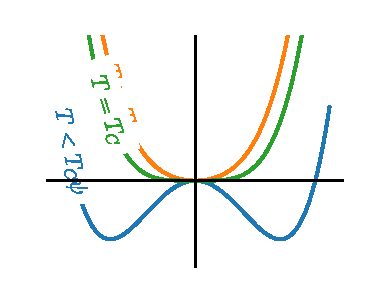
\includegraphics[width=\textwidth]{images/landau_free_energy}
		\caption{Ginzburg Landau free energy}
		\label{sfig:Ginzburg Landau free energy}
	\end{subfigure}
	\caption{Landau free energy and} 
	\label{fig:Landau free energy and Ginzburg-Landau free energy}
\end{figure}

Two minima for free energy function for \(T < T_C\).
With this, we can extract \(T_C\) from the knowledge of the dependence of \(\vert \psi \vert^2\) on \(T\) via a linear fit.
This is only valid for an area near \(T_C\) (where Landau theory holds), but can be used to get \(T_C\) from microscopic theories.

Going from a one to a \(n\)-component order parameters, OP acquires directions and magnitude.
Particularly important example: complex or two component order parameter in superfluids and superconductors:
\begin{equation}
	\psi = \psi_1 + \iu \psi_2 = \vert \psi \vert e^{\iu \phi}
\end{equation}
The Landau free energy takes the form:
\begin{equation}
	f[\psi] = r(\psi^* \psi) + \frac{u}{2} (\psi^* \psi)^2
\end{equation}
As before:
\begin{equation}
	r = a(T - T_C)
\end{equation}
shows the Landau free energy as function of \(\psi\).

Rotational symmetry, because free energy is independent of the global phase of the OP:
\begin{equation}
	f [\psi] = f [e^{\iu a } \psi]
\end{equation}
In this `Mexican hat' potential: order parameter can be rotated continuously from one broken-symmetry state to another.
If we want the phase to be rigid, we need to introduce an
There is a topological argument for the fact that the phase is rigid.
This leads to Ginzburg-Landau theory.
Will see later: well-defined phase is associated with persistent currents or superflow.

\paragraph{Ginzburg-Landau theory} \todo{Work over paragraph}

Landau theory: energy cost of a uniform order parameter, more general theory needs to account for inhomogenous order parameters, in which the amplitude varies or direction of order parameter is twisted -> GL theory.
First: one-component, `Ising' order parameter.
GL introduces additional energy \(\delta f \propto \vert \Delta \psi \vert^2\), \(f_{GL} [\psi, \Delta \psi] = \frac{s}{2} \vert \Delta \psi \vert^2 + f_L [\psi(s)]\), or in full:
\begin{equation}
	f_{GL} [\psi, \Delta \psi, h] = \frac{s}{2} (\Delta \psi)^2 + \frac{r}{2} \psi^2 + \frac{u}{4} \psi^4
\end{equation}
GL theory is only valid near critical point, where OP is small enough to permit leading-order expansion.
Dimensional analysis shows: \(\frac{s}{r} = L^2\) has dimension of length squared.
Length scale introduced by the gradient term: correlation length \gls{correlation length}
\begin{equation}
	\xi (T) = \sqrt{\frac{s}{\vert r(T) \vert}} = \xi_0 \left\vert 1 - \frac{T}{T_C} \right\vert^{-\frac{1}{2}}
\end{equation}
sets characteristic length scale of order-parameter fluctuations, where the zero temperature value
\begin{equation}
	\xi_0 = \xi (T = 0) = \sqrt{\frac{s}{\alpha T_C}}
\end{equation}
is the microscopic coherence length \gls{coherence length}.
Near transition \(\xi (T)\) diverges, but far from transition it becomes comparable with the coherence length.

\paragraph{Complex order and superflow} \todo{Work over paragraph}

Now: GL theory of complex or two-component order parameters, so superfluids and superconductors.
Heart of discussion: emergence of a `macroscopic wavefunction', where the microscopic field operators \(\hat{\psi}(x)\) acquire an expectation value:
\begin{equation}
	\braket{\hat{\psi} (x)} = \psi (x) = \vert \psi (x) \vert e^{\iu \theta(x)}
\end{equation}
Reminder: Field operators are the real space representations of creation/annihilation operators.
They can be thought of the super position of all ways of creating a particle at position \(x\) via the basis coefficients.

Magnitude determines density of particles in the superfluid:
\begin{equation}
	\vert \psi(x) \vert^2 = n_s (x)
\end{equation}
Density operator is
\begin{equation}
	\hat{\rho} = \hat{\psi} (x) \hat{\psi^{\dagger}} (x)
\end{equation}
so expectation value of that is the formula above.

Twist/gradient of phase determines superfluid velocity:
\begin{equation}
	\vb{v}_s (x) = \frac{\hbar}{m} \Delta \phi (x)
\end{equation}
We will derive this later in the chapter.
Counterintuitive from quantum mechanics: GL suggested that \(\Phi(x)\) is a macroscopic manifestation of a macroscopic number of particles condensed into precisely the same quantum state.
Emergent phenomenon, collective properties of mater not a-priori evident from microscopic physics.

GL free energy density for superfluid (with one added term in comparison to Landau energy):
\begin{equation}
	f_{GL} [\psi, \Delta \psi] = s \vert \Delta \psi \vert^2 + r \vert \psi \vert^2 + \frac{u}{2} \vert \psi \vert^4
\end{equation}
Compare with the energy density of a bosonic field (with a quarctic interaction):
\begin{align}
	H = \int \odif[order=D]{x} \frac{\hbar^2}{2m} \vert \Delta \psi \vert^2 + r \vert \psi \vert^2 + \frac{u}{2} \vert \psi \vert^4
\end{align}
Interpret GL free energy as energy density of a condensate of bosons in which the field operator behaves as a complex order parameter.
Gives interpretation of gradient term as kinetic energy:
\begin{equation}
	s \vert \Delta \psi \vert^2 = \frac{\hbar^2}{2m} \braket{\Delta \hat{\psi}^{\dagger} \Delta \hat{\psi}} \implies s = \frac{\hbar^2}{2m}
\end{equation}
As in Ising order: correlation length/GL-coherence length governs characteristic range of amplitude fluctuations of the order parameter:
\begin{equation}
	\xi = \sqrt{\frac{s}{\vert r \vert}} = \sqrt{\frac{\hbar^2}{2m \vert r \vert}} = \xi_0 (1 - \frac{T}{T_C})^{-\frac{1}{2}}
\end{equation}
where \(\xi_0 = \xi(T=0) = \sqrt{\frac{\hbar^2}{2 m a T_C}}\) is the coherence length.
Beyond this length scale: only phase fluctuations survive.
\todo{I dont know why that is. Can I support that somehow better? -> See Niklas thesis}

Freeze out fluctuations in amplitude (no \(x\)-dependence in amplitude) \(\psi(x) = \sqrt{n_s} e^{\iu \phi(x)}\), then \(\Delta \psi = \iu \Delta \phi \psi\) and \(\vert \Delta \psi \vert^2 = n_s (\Delta \phi)^2\), dependency of kinetic energy on the phase twist is (bringing it into the form \(\frac{m}{2} v^2\)):
\begin{equation}
	\frac{\hbar^2 n_s}{2m} (\Delta \phi)^2 = \frac{m n_s}{2} (\frac{\hbar}{m} \Delta \phi)^2
\end{equation}
So twist of phase results in increase in kinetic energy, associated with a superfluid velocity:
\begin{equation}
	\vb{v}_s = \frac{\hbar}{m} \Delta \phi
\end{equation}
(this is explained in detail later).

For interpretation of superfluid states: coherent states.
These are eigenstates of the field operator
\begin{equation}
	\hat{\psi}(x) \ket{\psi} = \psi (x) \ket{\psi} 
\end{equation}
and don't have a definite particle number.
Importantly, this small uncertainty in particle number enables a high degree of precision in phase (which is the property of a condensate).


\paragraph{Phase rigidity and superflow}

In GL theory, energy is sensitive to a twist of the phase.
Substitute \(\psi = \vert \psi \vert e^{\iu \phi}\) into GL free energy, gradient term is:
\begin{equation}
	\Delta \psi = (\Delta \vert \psi \vert + \iu \Delta \phi \vert \psi \vert) e^{\iu \phi}
\end{equation}
So:
\begin{equation}
	f_{GL}  = \frac{\hbar}{2m} \vert \psi \vert^2 (\Delta \phi)^2 + \left[ \frac{\hbar}{2m} (\Delta \vert \psi \vert)^2 + r \vert \psi \vert^2 + \frac{u}{2} \vert \psi \vert^4 \right]
\end{equation}
The second term resembles GL functional for an Ising order parameter, describes energy cost of variations in the magnitude of the order parameter.

\todo{Phase rigidity and superflow}


\subsection{Superconducting length scales}

From~\cite{wittBypassingLatticeBCSBEC2024}.

\todo{Better introduction}

In most materials: Cooper pairs do not carry finite center-of-mass momentum.
In presence of e.g.\ external fields or magnetism: SC states with FMP might arise.

Theory/procedure in the paper: enforce FMP states via constraints on pair-center-of-mass momentum \(\vb{q}\), access characteristic lenght scales \(\xi_0, \lambda_L\) through analysis of the momentum and temperature-dependent OP\@.
FF-type pairing with Cooper pairs carrying finite momentum:
\begin{equation}
	\psi_{\vb{q}} (\vb{r}) = \vert \psi_{\vb{q}} \vert e^{\iu \vb{q} \vb{r}}
\end{equation}
Then the free energy density is
\begin{equation}
	f_{GL} [\psi_{\vb{q}}] = \alpha \vert \psi_{\vb{q}} \vert^2 + \frac{b}{2} \vert \psi_{\vb{q}} \vert^4 + \frac{\hbar^2 q^2}{2 m^*} \vert \psi_{\vb{q}} \vert^2
\end{equation}
Stationary point of the system:
\begin{equation}
	\fdv{f_{GL}}{\psi_{\vb{q}}^*} = 2 \psi_{\vb{q}} \left[\alpha (1 - \xi^2 q^2) + b \vert \psi_{\vb{q}} \vert^2\right] = 0
\end{equation}
which results in the \(\vb{q}\)-dependence of the OP
\begin{equation}
	\vert \psi_{\vb{q}} \vert^2 = \vert \psi_{0} \vert^2 (1 - \xi(T)^2 q^2)
\end{equation}
For some value, SC order breaks down, \(\psi_{\vb{q}_c} = 0\), because the kinetic energy from phase modulation exceeds the gain in energy from pairing.
In GL theory: \(q_c = \xi(T)^{-1}\).
The temperature dependence of the OP and extracted \(\xi(T)\) gives access to the coherence length via
\begin{equation}
	\xi(T) = \xi_0 (1 - \frac{T}{T_C})^{-\frac{1}{2}}
\end{equation}
Specifically: take
\begin{equation}
	\xi(T) = \frac{1}{\sqrt{2} \vert \vb{Q} \vert}
\end{equation}
with \(\vb{Q}\) such that
\begin{equation}
	\vert \frac{\psi_{\vb{Q}}(T)}{\psi_0 (T)} \vert = \frac{1}{\sqrt{2}}
\end{equation}
The Cooper pair \cite{yuanSupercurrentDiodeEffect2022, shimanoHiggsModeSuperconductors2020}

\todo{Depairing current from FMP}

\todo{Full formula for supercurrent, with sum over orbitals}

\todo{DS from FMP}

\todo{Write more about the connection between all the things here}

\section{Bardeen-Coooper-Schrieffer Theory}\label{sec:bcs-theory}

First phenomenological description of SC: Fritz London in 1937 \cite{londonNewConceptionSupraconductivity1937}.
He was motivated by the discovery of the Meissner effect in 1933 \cite{meissnerNeuerEffektBei1933}, where magnetic flux inside of the superconductor is always pushed out in contrast to a perfectly conducting material, which would hold a `memory' of the magnetic field at the time of the phase transition. 
This suggests that transition to the SC state is reversible and a SC is not just the limiting case of a conductor with infinite conductivity, in which according to the Maxwell equations, the magnetic flux would not change.
Londons first descriptions is based on a one-particle wave function \(\phi (x)\).
He proposed that persistent supercurrent is a property of the ground state associated with its rigidity against the application of a field.

In 1950 \cite{ginzburgTheorySuperconductivity1950}: GL interpreted this wave function as a complex order parameter as explained in \cref{sec:Ginzburg-Landau theory of superconductivity}.

Following \cite[ch. 14]{colemanIntroductionManyBodyPhysics2015}.

\subsection{BCS Hamiltonian}

Microscopic description of SC: 1957 by John Bardeen, his postdoc Leon Cooper and the graduate in the group, J. Robert Schrieffer \cite{bardeenTheorySuperconductivity1957}.
Description is based on the fact that the Fermi sea is unstable towards development of bound pairs under arbitrarily small attraction \cite{cooperBoundElectronPairs1956}.
The final element in this description was the origin of the attractive interaction \(V_{{\vb{k}, \vb{k}^{\prime}}}\) between electrons, which Bardeen, Cooper and Schrieffer identified as a retarded electron-phonon interaction \cite{bardeenTheorySuperconductivity1957}.
BCS-Hamiltonian:
\begin{equation}\label{eq:BCS Hamiltonian}
	H_{\text{BCS}} = \sum_{\vb{k}\sigma} \epsilon_{\vb{k}\sigma} c_{\vb{k}\sigma}^{\dagger} c_{\vb{k}\sigma} + \sum_{\vb{k}, \vb{k}^{\prime}} V_{\vb{k}, \vb{k}^{\prime}} c_{\vb{k}\uparrow}^{\dagger} c_{-\vb{k}\downarrow}^{\dagger} c_{-\vb{k}^{\prime}\downarrow} c_{\vb{k}^{\prime}\uparrow}
\end{equation}
This Hamiltonian can be solved exactly using a mean field approach, because it involves an interaction at zero momentum and thus infinite range.
Order parameter in mean field BCS theory is the pairing amplitude
\begin{equation}
	\Delta = - \frac{U}{N_{\vb{k}}} \sum_{\vb{k}} \braket{c_{-\vb{k} \downarrow} c_{\vb{k} \uparrow}} = - U \braket{c_{-\vb{r}=0 \downarrow} c_{\vb{r=0} \uparrow}} \simeq U \Psi \;.
\end{equation}
More about mean field theory in \cref{ssec:attractive hubbard model}

A finite \(\Delta\) corresponds to the pairing introduced above: there is a finite expectation value for a coherent creation/annihilation of a pair of electrons with opposite momentum and spin.
A finite \(\Delta\) also introduces a band gap into the spectrum.
BCS theory brings multiple aspects together: concept of paired electrons with the pairing amplitude being the order parameter in SC, an explanation for the attractive interaction overcoming Coulomb repulsion and a model Hamiltonian that very elegantly captures the essential physics.

It is very successful in two ways: on the one hand it could quantitatively predict effects in the SCs known at the time, for example the Hebel-Slichter peak that was measured in 1957 \cite{hebelNuclearRelaxationSuperconducting1957, hebelNuclearSpinRelaxation1959} and the band gap measured by Giaever in 1960 \cite{giaeverStudySuperconductorsElectron1961}.  
On the other hand, it established electronic pairing as the microscopic mechanism behind SC, which holds still today even for high \(T_C\)/unconventional superconductors, so SCs that cannot be described by BCS theory \cite{zhouHightemperatureSuperconductivity2021}.

\todo{Other pairing interactions can be taken, gives explanations for a lot of different SCs}

\todo{Make graphic for Landau OP and BCS OP -> Formula for BCS OP!}

\subsection{Attractive Hubbard Model}\label{ssec:attractive hubbard model}

The Hubbard model is the simplest model for interacting electron systems.
It goes back to works by Hubbard \cite{hubbardElectronCorrelationsNarrow1963}, Kanamori \cite{kanamoriElectronCorrelationFerromagnetism1963} and Gutzweiler \cite{gutzwillerEffectCorrelationFerromagnetism1963}.
\begin{equation}
	H_{\mathrm{int}} = U \sum_{i} c_{i, \uparrow}^{\dagger} c_{i, \downarrow}^{\dagger} c_{i, \downarrow} c_{i, \uparrow}
\end{equation}
where \(U > 0\).

Besides 

\cite{qinHubbardModelComputational2022}

\todo{Some relevance of the repulsive Hubbard model}

This simple Hubbard model can be extended in a multitude of ways to model a variety of physical system.
In this work: extension to multiple orbitals (i.e. atoms in the unit cell for lattice systems) and an attractive interaction, i.e. a negative \(U\).
Physical motivation for taking a negative-U Hubbard model: electrons can experience a local attraction interaction, for example through electrons coupling with phononic degrees of freedom or with electronic excitations that can be described as bosons \cite{micnasSuperconductivityNarrowbandSystems1990}.
\todo{There are some more specific papers to the specific mechanisms (and also some more mechanism), could cite these here and say some more things}
The form of the interaction term is then: \todo{Order of operators? -> also in all other equations!}
\begin{equation}
	H_{\mathrm{int}} = -\sum_{i, \alpha} U_{\alpha} c_{i, \alpha, \uparrow}^{\dagger} c_{i, \alpha, \downarrow}^{\dagger} c_{i, \alpha, \downarrow} c_{i, \alpha, \uparrow}
	\label{eq:Hubbard interaction multiband}
\end{equation}
where \(\alpha\) counts orbitals and the minus sign in front is taken so that \(U > 0\) now corresponds to an attractive interaction (this is purely convention).

\paragraph{Multiband BCS Mean Field Theory}

There are a multitude of ways to derive a mean field description of a given interacting Hamiltonian.
Very rigorous in path integral formulations as saddle points, given for example in ref. \cite{colemanIntroductionManyBodyPhysics2015}.
A more intuitive way based on ref. \cite{bruusManyBodyQuantumTheory2004} discussed here looks at the operators and which one are small. 

Look at interaction term \cref{eq:Hubbard interaction multiband}.
Mean-field approximation (here specifically for superconductivity i.e. pairing): operators do not deviate much from their average value, i.e. the deviation operators \todo{there are other combinations, talk about that}
\begin{align}
	d_{i, \alpha} = c_{i, \alpha, \uparrow}^{\dagger} c_{i, \alpha, \downarrow}^{\dagger} - \braket{c_{i, \alpha, \uparrow}^{\dagger} c_{i, \alpha, \downarrow}^{\dagger}} \\
	e_{i, \alpha} = c_{i, \alpha, \downarrow} c_{i, \alpha, \uparrow} - \braket{c_{i, \alpha, \downarrow} c_{i, \alpha, \uparrow}}
\end{align}
are small (dont contribute much to expectation values and correlation functions), so that in the interaction part of the Hamiltonian
\begin{align}
	H_{\mathrm{int}} &= -\sum_{i, \alpha} U_{\alpha} c_{i, \alpha, \uparrow}^{\dagger} c_{i, \alpha, \downarrow}^{\dagger} c_{i, \alpha, \downarrow} c_{i, \alpha, \uparrow} \\
	&= -\sum_{i, \alpha} U_{\alpha} 
	\left( d_{i, \alpha}^{\dagger} + \braket{c_{i, \alpha, \uparrow}^{\dagger} c_{i, \alpha, \downarrow}^{\dagger}} \right)
	\left( e_{i, \alpha} + \braket{c_{i, \alpha, \downarrow} c_{i, \alpha, \uparrow}} \right) \\
	&= -\sum_{i, \alpha} U_{\alpha} (
		d_{i, \alpha} e_{i, \alpha}
		+ d_{i, \alpha} \braket{c_{i, \alpha, \downarrow} c_{i, \alpha, \uparrow}}
		+ e_{i, \alpha} \braket{c_{i, \alpha, \uparrow}^{\dagger} c_{i, \alpha, \downarrow}^{\dagger}} \\
		&+ \braket{c_{i, \alpha, \uparrow}^{\dagger} c_{i, \alpha, \downarrow}^{\dagger}} \braket{c_{i, \alpha, \downarrow} c_{i, \alpha, \uparrow}} )
\end{align}
the first term is quadratic in the deviation and can be neglected.
Thus arrive at the approximation
\begin{align}
	H_{\mathrm{int}} &\approx -\sum_{i, \alpha} U_{\alpha} \left(
	d_{i, \alpha} \braket{c_{i, \alpha, \downarrow} c_{i, \alpha, \uparrow}}
	+ e_{i, \alpha} \braket{c_{i, \alpha, \uparrow}^{\dagger} c_{i, \alpha, \downarrow}^{\dagger}}
	+ \braket{c_{i, \alpha, \uparrow}^{\dagger} c_{i, \alpha, \downarrow}^{\dagger}} \braket{c_{i, \alpha, \downarrow} c_{i, \alpha, \uparrow}}
	\right) \\
	&= -\sum_{i, \alpha} U_{\alpha} (
		c_{i, \alpha, \uparrow}^{\dagger} c_{i, \alpha, \downarrow}^{\dagger} \braket{c_{i, \alpha, \downarrow} c_{i, \alpha, \uparrow}}
		+ c_{i, \alpha, \downarrow} c_{i, \alpha, \uparrow} \braket{c_{i, \alpha, \uparrow}^{\dagger} c_{i, \alpha, \downarrow}^{\dagger}} \\	
	&- \braket{c_{i, \alpha, \uparrow}^{\dagger} c_{i, \alpha, \downarrow}^{\dagger}} \braket{c_{i, \alpha, \downarrow} c_{i, \alpha, \uparrow}} ) \\
	&= 
\end{align}
with the expectation values
\begin{equation}
	\Delta
\end{equation}

\todo{General multi-band mean field theory theory}

\todo{Mean field with finite momentum}


\begin{align}
	H_{\mathrm{int}} \approx \sum_{\alpha, \vb{k}} (\Delta_{\alpha} c_{\vb{k} \alpha \uparrow}^{\dagger} c_{-\vb{k} \alpha \downarrow}^{\dagger} + \Delta_{\alpha}^* c_{-\vb{k} \alpha \downarrow} c_{\vb{k} \alpha \uparrow})
\end{align}


Fourier transformation:
\begin{equation}
	H_{int} = - \frac{1}{N^2} \sum_{\alpha, \vb{k}_{1, 2, 3, 4}} U_{\alpha} e^{\iu (\vb{k}_1 + \vb{k}_4 - \vb{k}_1 - \vb{k}_3) r_{i \alpha}}  c_{\vb{k}_1 \alpha \uparrow}^{\dagger} c_{\vb{k}_3 \alpha \downarrow}^{\dagger} c_{\vb{k}_2 \alpha \downarrow} c_{\vb{k}_4 \alpha \uparrow}
\end{equation}
Impose zero-momentum pairing: \(\vb{k}_1 + \vb{k}_3 = 0\) and \(\vb{k}_2 + \vb{k}_4 = 0\):
\begin{align}
	H_{int} = - \sum_{\alpha, \vb{k}, \vb{k}^{\prime}} U_{\alpha} c_{\vb{k} \alpha \uparrow}^{\dagger} c_{-\vb{k} \alpha \downarrow}^{\dagger} c_{-\vb{k}^{\prime} \alpha \downarrow} c_{\vb{k}^{\prime} \alpha \uparrow}
\end{align}
Mean-field approximation:
\begin{align}
	H_{int} \approx \sum_{\alpha, \vb{k}} (\Delta_{\alpha} c_{\vb{k} \alpha \uparrow}^{\dagger} c_{-\vb{k} \alpha \downarrow}^{\dagger} + \Delta_{\alpha}^* c_{-\vb{k} \alpha \downarrow} c_{\vb{k} \alpha \uparrow})
\end{align}
with
\begin{align}
	\Delta_{\alpha} &= - U_{\alpha} \sum_{\vb{k}^{\prime}} \braket{c_{-\vb{k}^{\prime} \alpha \downarrow} c_{\vb{k}^{\prime} \alpha \uparrow}} \\
	\Delta_{\alpha}^* &= - U_{\alpha} \sum_{\vb{k}^{\prime}} \braket{c_{\vb{k}^{\prime} \alpha \uparrow}^{\dagger} c_{-\vb{k}^{\prime} \alpha \downarrow}^{\dagger}}
\end{align}
This gives the BCS mean field Hamiltonian:
\begin{align}
	H_{BCS} = \sum_{\vb{k} \alpha \beta \sigma} [H_{0, \sigma} (\vb{k})]_{\alpha \beta} c_{\vb{k} \alpha \sigma}^{\dagger} c_{\vb{k} \beta \sigma}
	-\mu \sum_{\vb{k} \alpha \sigma} n_{\vb{k} \alpha \sigma}
	+ \sum_{\alpha, \vb{k}} (\Delta_{\alpha} c_{\vb{k} \alpha \uparrow}^{\dagger} c_{-\vb{k} \alpha \downarrow}^{\dagger} + \Delta_{\alpha}^* c_{-\vb{k} \alpha \downarrow} c_{\vb{k} \alpha \uparrow})
\end{align}
with Nambu spinor

\todo{Nambu spinor}

\begin{equation}
	\Psi_{\vb{k}} =
	\begin{pmatrix}
		c_{1, \vb{k} \uparrow} \\
		c_{2, \vb{k} \uparrow} \\
		c_{3, \vb{k} \uparrow} \\
		c_{1, -\vb{k} \downarrow}^{\dagger} \\
		c_{2, -\vb{k} \downarrow}^{\dagger} \\
		c_{3, -\vb{k} \downarrow}^{\dagger} \\
	\end{pmatrix}
\end{equation}
we have:
\begin{equation}
	H_{MF} = \sum_{\vb{k}} \Psi_{\vb{k}}^{\dagger} \mathcal{H} (\vb{k}) \Psi_{\vb{k}}
\end{equation}
with
\begin{equation}
	\mathcal{H} (\vb{k}) =
	\begin{pmatrix}
		H_{0, \uparrow} (\vb{k}) - \mu & \Delta \\
		\Delta^{\dagger} & - H_{0, \downarrow}^* (-\vb{k}) + \mu
	\end{pmatrix}
\end{equation}
with \(H_{0, \sigma}\) being the F.T. of the kinetic term and \(\Delta = diag(\Delta_1, \Delta_2, \Delta_3)\).


\paragraph{Self-consistency}

Formula for OP using the Bogoliubov operators
\begin{equation}
	\Delta_{\alpha} = -U
\end{equation}

\todo{How to solve mean field theory self-consistently}

\paragraph{Finite momentum}

To include finite momentum, take the ansatz of a Fulde-Ferrel (FF) type pairing \cite{kinnunenFuldeFerrellLarkin2018}:
\begin{equation}
	\Delta
\end{equation}

\todo{How to include finite momentum}

\section{Dynamical Mean-Field Theory (DMFT)}\label{sec:Dynamical Mean-Field Theory}

\subsection{Green's Function Formalism}



Following~\cite{bruusManyBodyQuantumTheory2004}

\todo{Work over the paragraph}

Green's functions: method to encode influence of many-body effects on propagation of particles in a system.

Have different kinds of Green's functions, for example the retarded Green's function:
\begin{equation}
	G^R (\vb{r}\sigma t, \vb{r}^{\prime} \sigma^{\prime} t^{\prime}) = -\iu \Theta(t- t^{\prime}) \braket{ \{c_{\vb{r} \sigma} (t), c_{\vb{r} \sigma}^{\dagger} (t^{\prime})\}}
\end{equation}
They give the amplitude of a particle inserted at point \(\vb{r}^{\prime}\) at time \(t^{\prime}\) to propagate to position \(\vb{r}\) at time \(t\).
For time-independent Hamiltonians and systems in equilibrium, the GFs only depend on time differences:
\begin{equation}
	G^R (\vb{r}\sigma t, \vb{r}^{\prime} \sigma^{\prime} t^{\prime}) = G^R (\vb{r} \sigma, \vb{r}^{\prime} \sigma^{\prime}, t - t^{\prime})
\end{equation}
So we can take \(t^{\prime} = 0\) and consider \(t\) as the only free variable:
\begin{equation}
	G^R (\vb{r}\sigma, \vb{r}^{\prime} \sigma^{\prime}, t) = -\iu \Theta(t) \braket{ \{c_{\vb{r} \sigma} (t), c_{\vb{r} \sigma}^{\dagger} (0)\}}
\end{equation}
In a translation invariant system: can use \(\vb{k}\) as a natural basis set:
\begin{equation}
	G^R (\vb{k}, \sigma, \sigma^{\prime} t) = -\iu \Theta(t- t^{\prime}) \braket{ \{c_{\vb{k} \sigma} (t), c_{\vb{k} \sigma^{\prime}}^{\dagger} (0)\}}
\end{equation}
Define Fourier-transform:
\begin{equation}
	G^R (\vb{k}, \sigma, \sigma^{\prime}, \omega) = \int_{-\infty}^{\infty} \odif{t} G^R (\vb{k}, \sigma, \sigma^{\prime} t)
\end{equation}
Can define the spectral function from this:
\begin{equation}
	A(\vb{k} \sigma, \omega) = -2 \Im G^R (\vb{k} \sigma, \omega)
\end{equation}
Looking at the diagonal elements of \(G^R\) here.
The spectral function can be thought of as the energy resolution of a particle with energy \(\omega\).
This mean, for non-interacting systems, the spectral function is a delta-function around the single-particle energies:
\begin{equation}
	A_0 (\vb{k} \sigma, \omega) = 2\pi \delta (\omega - \epsilon_{\vb{k} \sigma})
\end{equation}
For interacting systems this is not true, but \(A\) can still be peaked.

\todo{Show GFs can be related to observables}

Mathematical technique to calculate retarded GFs involves defining GFs on imaginary times \gls{imaginary time}:
\begin{equation}
	t \to -\iu \tau
\end{equation}
where \(\tau\) is real and has the dimension time.
This enables the simultaneous expansion of exponential \(e^{-\beta H}\) coming from the thermodynamic average and \(e^{-\iu H t}\) coming from the time evolution of operators.

Define imaginary time/Matsubara GF \gls{matsubara correlation function}:
\begin{equation}
	\mathcal{C}_{A B} (\tau, 0) = - \Braket{T_{\tau} (A(\tau) B(0))}
\end{equation}
with time-ordering operator in imaginary time:
\begin{equation}
	T_{\tau} (A(\tau) B(\tau^{\prime})) = \Theta(\tau - \tau^{\prime}) A(\tau) B(\tau^{\prime}) \pm \Theta(\tau^{\prime} - \tau) B(\tau^{\prime}) A(\tau)
\end{equation}
so that operators with later `times' go to the left.

Can prove from properties of Matsubara GF, that they are only defined for
\begin{equation}
	-\beta < \tau < \beta
\end{equation}
Due to this, the Fourier transform of the Matsubara GF is defined on discrete values:
\begin{equation}
	\mathcal{C}_{A B} (\iu \omega_n) = \int_{0}^{\beta} \odif{\tau}
\end{equation}
with fermionic/bosonic Matsubara frequencies
\begin{equation}
	\omega_n =
	\begin{cases}
		\frac{2n \pi}{\beta} \, \text{for bosons} \\
		\frac{(2n + 1)\pi}{\beta} \, \text{for fermions}
	\end{cases}
\end{equation}

\todo{How to resolve ambiguity at borders of integral}

It turns out that Matsubara GFs and retarded GFs can be generated from a common function \(\mathcal{C}_{AB} (z)\) that is defined on the entire complex plane except for the real axis.
So we can get the retarded GF \(\mathcal{C}_{AB}^R (\omega)\) by analytic continuation:
\begin{equation}
	\mathcal{C}_{AB}^R (\omega) = \mathcal{C}_{AB} (\iu \omega_n \to \omega + \iu \eta)
\end{equation}
\todo{What is the eta there -> need to define it in retarded GF}
So in particular the extrapolation of the Matsubara GF to zero is proportional to the density of states at the chemical potential.
Gapped: density is zero (Matsubara GF goes to 0), metal: density is finite (Matsubara GF goes to finite value) ~\cite[8.3.4]{bruusManyBodyQuantumTheory2004}.

\todo{single-particle Matsubara GF}

\subsection{Perturbation theory, Dyson equation}

\todo{Short introduction to diagrams}

\todo{Self energy}

\todo{Dyson equation}

Dyson equation:
\begin{equation}
	\mathcal{G}_{\sigma} (\vb{k}, \iu \omega_n) = \frac{\mathcal{G}_{\sigma}^0 (\vb{k}, \iu \omega_n)}{1 - \mathcal{G}_{\sigma}^0 (\vb{k}, \iu \omega_n) \Sigma_{\sigma} (\vb{k}, \iu \omega_n)} = \frac{1}{\iu \omega_n - \xi_{\vb{k} - \Sigma_{\sigma} (\vb{k}, \iu \omega_n)}}
\end{equation}


\subsection{Nambu-Gorkov GF}

Introduction following~\cite[ch. 14.7]{colemanIntroductionManyBodyPhysics2015}

\todo{More general introduction into NG GFs, how they look like, what they describe etc.}

Order parameter can be chosen as the anomalous GF:
\begin{equation}
	\Psi = F^{\mathrm{loc}} (\tau = 0^-)
\end{equation}
or the superconducting gap
\begin{equation}
	\Delta = Z \Sigma^{\mathrm{AN}}
\end{equation}
that can be calculated from the anomalous self-energy \(\Sigma^{\mathrm{AN}}\) and quasiparticle weight \(Z\)
\todo{Sources for these?}

\todo{How to get quasiparticle weight?}

\subsection{DMFT}

Following \cite{georgesDynamicalMeanfieldTheory1996}.

Most general non-interacting electronic Hamiltonian in second quantization:
\begin{equation}
	H_0 = \sum_{i, j, \sigma}
\end{equation}
with lattice coordinates \(i, j\) and spin \(\sigma\).

One particle Green's function (many-body object, coming from the Hubbard model):
\begin{equation}
	G(\vb{k}, \iu \omega_n) = \frac{1}{\iu \omega_n + \mu - \epsilon_{\vb{k}} - \Sigma(\vb{k}, \iu \omega_n)}
\end{equation}
with the self energy \(\Sigma(\iu \omega_n)\) coming from the solution of the effect on-site problem:

The Dyson equation
\begin{equation}
	G(\vb{k}, \iu \omega_n) = \left( G_0 (\vb{k}, \iu \omega_n) - \Sigma(\vb{k}, \iu \omega_n)\right)^{-1}
\end{equation}
relates the non-interacting Greens function \(G_0 (\vb{k}, \iu \omega_n)\) and the fully-interacting Greens function \(G (\vb{k}, \iu \omega_n)\) (inversion of a matrix!).

\end{document}
